% Options for packages loaded elsewhere
\PassOptionsToPackage{unicode}{hyperref}
\PassOptionsToPackage{hyphens}{url}
\PassOptionsToPackage{dvipsnames,svgnames,x11names}{xcolor}
%
\documentclass[
  letterpaper,
  DIV=11,
  numbers=noendperiod]{scrartcl}

\usepackage{amsmath,amssymb}
\usepackage{iftex}
\ifPDFTeX
  \usepackage[T1]{fontenc}
  \usepackage[utf8]{inputenc}
  \usepackage{textcomp} % provide euro and other symbols
\else % if luatex or xetex
  \usepackage{unicode-math}
  \defaultfontfeatures{Scale=MatchLowercase}
  \defaultfontfeatures[\rmfamily]{Ligatures=TeX,Scale=1}
\fi
\usepackage{lmodern}
\ifPDFTeX\else  
    % xetex/luatex font selection
\fi
% Use upquote if available, for straight quotes in verbatim environments
\IfFileExists{upquote.sty}{\usepackage{upquote}}{}
\IfFileExists{microtype.sty}{% use microtype if available
  \usepackage[]{microtype}
  \UseMicrotypeSet[protrusion]{basicmath} % disable protrusion for tt fonts
}{}
\makeatletter
\@ifundefined{KOMAClassName}{% if non-KOMA class
  \IfFileExists{parskip.sty}{%
    \usepackage{parskip}
  }{% else
    \setlength{\parindent}{0pt}
    \setlength{\parskip}{6pt plus 2pt minus 1pt}}
}{% if KOMA class
  \KOMAoptions{parskip=half}}
\makeatother
\usepackage{xcolor}
\setlength{\emergencystretch}{3em} % prevent overfull lines
\setcounter{secnumdepth}{-\maxdimen} % remove section numbering
% Make \paragraph and \subparagraph free-standing
\ifx\paragraph\undefined\else
  \let\oldparagraph\paragraph
  \renewcommand{\paragraph}[1]{\oldparagraph{#1}\mbox{}}
\fi
\ifx\subparagraph\undefined\else
  \let\oldsubparagraph\subparagraph
  \renewcommand{\subparagraph}[1]{\oldsubparagraph{#1}\mbox{}}
\fi


\providecommand{\tightlist}{%
  \setlength{\itemsep}{0pt}\setlength{\parskip}{0pt}}\usepackage{longtable,booktabs,array}
\usepackage{calc} % for calculating minipage widths
% Correct order of tables after \paragraph or \subparagraph
\usepackage{etoolbox}
\makeatletter
\patchcmd\longtable{\par}{\if@noskipsec\mbox{}\fi\par}{}{}
\makeatother
% Allow footnotes in longtable head/foot
\IfFileExists{footnotehyper.sty}{\usepackage{footnotehyper}}{\usepackage{footnote}}
\makesavenoteenv{longtable}
\usepackage{graphicx}
\makeatletter
\def\maxwidth{\ifdim\Gin@nat@width>\linewidth\linewidth\else\Gin@nat@width\fi}
\def\maxheight{\ifdim\Gin@nat@height>\textheight\textheight\else\Gin@nat@height\fi}
\makeatother
% Scale images if necessary, so that they will not overflow the page
% margins by default, and it is still possible to overwrite the defaults
% using explicit options in \includegraphics[width, height, ...]{}
\setkeys{Gin}{width=\maxwidth,height=\maxheight,keepaspectratio}
% Set default figure placement to htbp
\makeatletter
\def\fps@figure{htbp}
\makeatother

\usepackage{booktabs}
\usepackage{longtable}
\usepackage{array}
\usepackage{multirow}
\usepackage{wrapfig}
\usepackage{float}
\usepackage{colortbl}
\usepackage{pdflscape}
\usepackage{tabu}
\usepackage{threeparttable}
\usepackage{threeparttablex}
\usepackage[normalem]{ulem}
\usepackage{makecell}
\usepackage{xcolor}
\KOMAoption{captions}{tableheading}
\makeatletter
\makeatother
\makeatletter
\makeatother
\makeatletter
\@ifpackageloaded{caption}{}{\usepackage{caption}}
\AtBeginDocument{%
\ifdefined\contentsname
  \renewcommand*\contentsname{Table of contents}
\else
  \newcommand\contentsname{Table of contents}
\fi
\ifdefined\listfigurename
  \renewcommand*\listfigurename{List of Figures}
\else
  \newcommand\listfigurename{List of Figures}
\fi
\ifdefined\listtablename
  \renewcommand*\listtablename{List of Tables}
\else
  \newcommand\listtablename{List of Tables}
\fi
\ifdefined\figurename
  \renewcommand*\figurename{Figure}
\else
  \newcommand\figurename{Figure}
\fi
\ifdefined\tablename
  \renewcommand*\tablename{Table}
\else
  \newcommand\tablename{Table}
\fi
}
\@ifpackageloaded{float}{}{\usepackage{float}}
\floatstyle{ruled}
\@ifundefined{c@chapter}{\newfloat{codelisting}{h}{lop}}{\newfloat{codelisting}{h}{lop}[chapter]}
\floatname{codelisting}{Listing}
\newcommand*\listoflistings{\listof{codelisting}{List of Listings}}
\makeatother
\makeatletter
\@ifpackageloaded{caption}{}{\usepackage{caption}}
\@ifpackageloaded{subcaption}{}{\usepackage{subcaption}}
\makeatother
\makeatletter
\@ifpackageloaded{tcolorbox}{}{\usepackage[skins,breakable]{tcolorbox}}
\makeatother
\makeatletter
\@ifundefined{shadecolor}{\definecolor{shadecolor}{rgb}{.97, .97, .97}}
\makeatother
\makeatletter
\makeatother
\makeatletter
\makeatother
\ifLuaTeX
  \usepackage{selnolig}  % disable illegal ligatures
\fi
\IfFileExists{bookmark.sty}{\usepackage{bookmark}}{\usepackage{hyperref}}
\IfFileExists{xurl.sty}{\usepackage{xurl}}{} % add URL line breaks if available
\urlstyle{same} % disable monospaced font for URLs
\hypersetup{
  pdftitle={Analysis of SEAMAP data for the western GoM for all years (1983 - 2022) and summer sampling months of June, July, and August},
  pdfauthor={Shayna A. Sura},
  colorlinks=true,
  linkcolor={blue},
  filecolor={Maroon},
  citecolor={Blue},
  urlcolor={Blue},
  pdfcreator={LaTeX via pandoc}}

\title{Analysis of SEAMAP data for the western GoM for all years (1983 -
2022) and summer sampling months of June, July, and August}
\author{Shayna A. Sura}
\date{}

\begin{document}
\maketitle
\ifdefined\Shaded\renewenvironment{Shaded}{\begin{tcolorbox}[boxrule=0pt, borderline west={3pt}{0pt}{shadecolor}, frame hidden, sharp corners, interior hidden, enhanced, breakable]}{\end{tcolorbox}}\fi

\hypertarget{tropicalization-of-gulf-of-mexico-fish-communities}{%
\section{Tropicalization of Gulf of Mexico Fish
Communities}\label{tropicalization-of-gulf-of-mexico-fish-communities}}

\hypertarget{analysis-of-seamap-trawl-data}{%
\subsection{Analysis of SEAMAP Trawl
Data}\label{analysis-of-seamap-trawl-data}}

\hypertarget{data-subset-western-gom-stations-for-summer-trawls-june-july-august-in-years-1983---2022}{%
\subsubsection{Data Subset: western GoM stations for summer trawls
(June, July, August) in years 1983 -
2022}\label{data-subset-western-gom-stations-for-summer-trawls-june-july-august-in-years-1983---2022}}

\newpage

\textbf{Table 1.} Number of trawl stations for each year of data and the
fall months during which sampling took place (6 = June, 7 = July, 8 =
August). \begingroup\fontsize{10}{12}\selectfont

\begin{longtable*}[t]{rrl}
\toprule
year & \# of trawls & months\\
\midrule
1983 & 381 & 8; 6; 7\\
1984 & 291 & 6; 7; 8\\
1985 & 404 & 6; 7; 8\\
1986 & 270 & 6; 7\\
1987 & 652 & 6; 7\\
\addlinespace
1988 & 542 & 6; 7\\
1989 & 389 & 6; 7\\
1990 & 435 & 6; 7; 8\\
1991 & 418 & 6; 7\\
1992 & 407 & 7; 6\\
\addlinespace
1993 & 444 & 8; 6; 7\\
1994 & 394 & 6; 7; 8\\
1995 & 370 & 6; 8; 7\\
1996 & 374 & 7; 6; 8\\
1997 & 371 & 6; 7; 8\\
\addlinespace
1998 & 335 & 6; 7\\
1999 & 377 & 6; 7; 8\\
2000 & 377 & 6; 7\\
2001 & 269 & 7; 6\\
2002 & 372 & 6; 7\\
\addlinespace
2003 & 303 & 6; 7\\
2004 & 363 & 6; 7\\
2005 & 300 & 6; 7; 8\\
2006 & 375 & 6; 7; 8\\
2007 & 353 & 6; 7; 8\\
\addlinespace
2008 & 377 & 6; 8; 7\\
2009 & 476 & 6; 8; 7\\
2010 & 319 & 6; 8; 7\\
2011 & 265 & 6; 7\\
2012 & 293 & 6; 7\\
\addlinespace
2013 & 250 & 7; 6\\
2014 & 259 & 6; 7\\
2015 & 188 & 6; 7\\
2016 & 179 & 6; 7\\
2017 & 178 & 6; 7\\
\addlinespace
2018 & 149 & 6; 7\\
2019 & 166 & 6; 7\\
2021 & 127 & 6; 7\\
2022 & 133 & 6; 8\\
\bottomrule
\end{longtable*}
\endgroup{}

\newpage

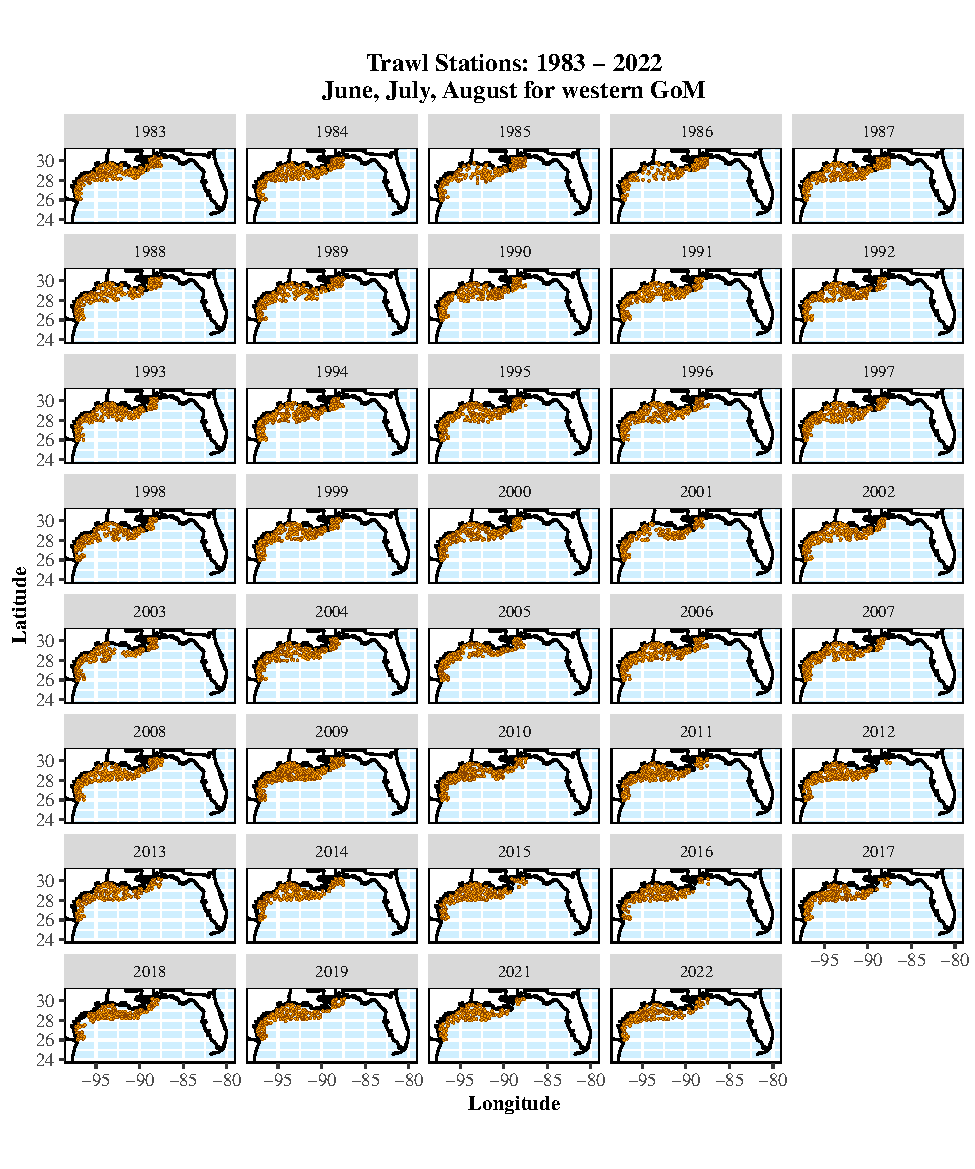
\includegraphics{9_westernGoM_summer_files/figure-pdf/map the trawl station locations-1.pdf}

\textbf{Figure 1.} Trawl sampling locations for the western GoM for each
year of data collection for this subset of data (1983-2022 summer
sampling in months of June, July, and August).

There are 513 fish species that were caught in trawls in this subset of
data.

Of those 513 fish species, only 294 of them had gCOB values for at least
5 years. For these fish species, linear models were constructed to test
if their latitude and longitude gCOBs had shifted over time.

\newpage

\textbf{Table 2.} The number of fish species that have significantly
shifted latitudinally or longitudinally based upon their gCOBs.

\begin{longtable}[]{@{}
  >{\centering\arraybackslash}p{(\columnwidth - 14\tabcolsep) * \real{0.1045}}
  >{\centering\arraybackslash}p{(\columnwidth - 14\tabcolsep) * \real{0.0373}}
  >{\centering\arraybackslash}p{(\columnwidth - 14\tabcolsep) * \real{0.2090}}
  >{\centering\arraybackslash}p{(\columnwidth - 14\tabcolsep) * \real{0.1119}}
  >{\centering\arraybackslash}p{(\columnwidth - 14\tabcolsep) * \real{0.1119}}
  >{\centering\arraybackslash}p{(\columnwidth - 14\tabcolsep) * \real{0.2164}}
  >{\centering\arraybackslash}p{(\columnwidth - 14\tabcolsep) * \real{0.1045}}
  >{\centering\arraybackslash}p{(\columnwidth - 14\tabcolsep) * \real{0.1045}}@{}}
\toprule\noalign{}
\begin{minipage}[b]{\linewidth}\centering
climate zone
\end{minipage} & \begin{minipage}[b]{\linewidth}\centering
n
\end{minipage} & \begin{minipage}[b]{\linewidth}\centering
significant latitude shift
\end{minipage} & \begin{minipage}[b]{\linewidth}\centering
North shifted
\end{minipage} & \begin{minipage}[b]{\linewidth}\centering
South shifted
\end{minipage} & \begin{minipage}[b]{\linewidth}\centering
significant longitude shift
\end{minipage} & \begin{minipage}[b]{\linewidth}\centering
West shifted
\end{minipage} & \begin{minipage}[b]{\linewidth}\centering
East shifted
\end{minipage} \\
\midrule\noalign{}
\endhead
\bottomrule\noalign{}
\endlastfoot
deep-water & 12 & 5 & 1 & 4 & 3 & 3 & 0 \\
subtropical & 203 & 47 & 10 & 37 & 53 & 44 & 9 \\
temperate & 5 & 0 & 0 & 0 & 1 & 1 & 0 \\
tropical & 74 & 24 & 3 & 21 & 25 & 22 & 3 \\
\end{longtable}

\textbf{Table 3.} The tropical fish species that have significantly
shifted their geographical center of biomass (gCOB) over time.

\begingroup\fontsize{9.5}{11.5}\selectfont

\begin{longtable*}[t]{ccccc}
\toprule
index & north & south & west & east\\
\midrule
\em{1} & \em{Pareques acuminatus} & \em{Bellator brachychir} & \em{Bellator brachychir} & \em{Pareques acuminatus}\\
\em{2} & \em{Prionotus roseus} & \em{Citharichthys spilopterus} & \em{Citharichthys spilopterus} & \em{Prionotus roseus}\\
\em{3} & \em{Rypticus saponaceus} & \em{Diplectrum bivittatum} & \em{Diplectrum bivittatum} & \em{Rypticus saponaceus}\\
\em{4} & \em{} & \em{Engyophrys senta} & \em{Echiophis punctifer} & \em{}\\
\em{5} & \em{} & \em{Gobionellus hastatus} & \em{Engyophrys senta} & \em{}\\
\addlinespace
\em{6} & \em{} & \em{Gymnothorax kolpos} & \em{Gobioides broussonnetii} & \em{}\\
\em{7} & \em{} & \em{Lepophidium brevibarbe} & \em{Gymnothorax kolpos} & \em{}\\
\em{8} & \em{} & \em{Lepophidium jeannae} & \em{Lepophidium brevibarbe} & \em{}\\
\em{9} & \em{} & \em{Neobythites gillii} & \em{Lepophidium jeannae} & \em{}\\
\em{10} & \em{} & \em{Ogcocephalus declivirostris} & \em{Ogcocephalus declivirostris} & \em{}\\
\addlinespace
\em{11} & \em{} & \em{Ogcocephalus nasutus} & \em{Ogcocephalus nasutus} & \em{}\\
\em{12} & \em{} & \em{Ophidion holbrookii} & \em{Ophidion holbrookii} & \em{}\\
\em{13} & \em{} & \em{Ophidion welshi} & \em{Ophidion welshi} & \em{}\\
\em{14} & \em{} & \em{Pontinus longispinis} & \em{Pontinus longispinis} & \em{}\\
\em{15} & \em{} & \em{Porichthys plectrodon} & \em{Prionotus longispinosus} & \em{}\\
\addlinespace
\em{16} & \em{} & \em{Prionotus longispinosus} & \em{Rhynchoconger flavus} & \em{}\\
\em{17} & \em{} & \em{Rhynchoconger flavus} & \em{Saurida normani} & \em{}\\
\em{18} & \em{} & \em{Saurida normani} & \em{Scorpaena calcarata} & \em{}\\
\em{19} & \em{} & \em{Serranus atrobranchus} & \em{Serranus atrobranchus} & \em{}\\
\em{20} & \em{} & \em{Syacium gunteri} & \em{Syacium gunteri} & \em{}\\
\addlinespace
\em{21} & \em{} & \em{Trichopsetta ventralis} & \em{Synodus foetens} & \em{}\\
\em{22} & \em{} & \em{} & \em{Trichopsetta ventralis} & \em{}\\
\bottomrule
\end{longtable*}
\endgroup{}

\newpage

\textbf{Table 4.} The subtropical fish species that have significantly
shifted their geographical center of biomass (gCOB) over time.

\begin{longtable*}[t]{ccccc}
\toprule
index & north & south & west & east\\
\midrule
\em{1} & \em{Bembrops gobioides} & \em{Ariopsis felis} & \em{Ancylopsetta quadrocellata} & \em{Centropristis ocyurus}\\
\em{2} & \em{Centropristis ocyurus} & \em{Bagre marinus} & \em{Archosargus probatocephalus} & \em{Decapterus macarellus}\\
\em{3} & \em{Decapterus macarellus} & \em{Bathyanthias mexicana} & \em{Ariopsis felis} & \em{Halieutichthys aculeatus}\\
\em{4} & \em{Diplectrum formosum} & \em{Bollmannia communis} & \em{Astroscopus y-graecum} & \em{Larimus fasciatus}\\
\em{5} & \em{Halieutichthys aculeatus} & \em{Bregmaceros atlanticus} & \em{Bagre marinus} & \em{Otophidium omostigma}\\
\addlinespace
\em{6} & \em{Hemicaranx amblyrhynchus} & \em{Brotula barbata} & \em{Bathyanthias mexicana} & \em{Paralichthys albigutta}\\
\em{7} & \em{Leiostomus xanthurus} & \em{Caulolatilus cyanops} & \em{Bollmannia communis} & \em{Rostroraja eglanteria}\\
\em{8} & \em{Paralichthys albigutta} & \em{Caulolatilus intermedius} & \em{Bregmaceros atlanticus} & \em{Sphoeroides dorsalis}\\
\em{9} & \em{Selene setapinnis} & \em{Centropristis philadelphica} & \em{Brotula barbata} & \em{Xyrichtys novacula}\\
\em{10} & \em{Xyrichtys novacula} & \em{Cyclopsetta chittendeni} & \em{Caulolatilus intermedius} & \em{}\\
\addlinespace
\em{11} & \em{} & \em{Dorosoma petenense} & \em{Centropristis philadelphica} & \em{}\\
\em{12} & \em{} & \em{Epinephelus flavolimbatus} & \em{Citharichthys macrops} & \em{}\\
\em{13} & \em{} & \em{Etropus crossotus} & \em{Cyclopsetta chittendeni} & \em{}\\
\em{14} & \em{} & \em{Gymnachirus melas} & \em{Etropus crossotus} & \em{}\\
\em{15} & \em{} & \em{Gymnachirus texae} & \em{Gymnachirus texae} & \em{}\\
\addlinespace
\em{16} & \em{} & \em{Gymnothorax nigromarginatus} & \em{Gymnothorax nigromarginatus} & \em{}\\
\em{17} & \em{} & \em{Hirundichthys rondeletii} & \em{Hirundichthys rondeletii} & \em{}\\
\em{18} & \em{} & \em{Histrio histrio} & \em{Histrio histrio} & \em{}\\
\em{19} & \em{} & \em{Hoplunnis macrurus} & \em{Hoplunnis macrurus} & \em{}\\
\em{20} & \em{} & \em{Lutjanus campechanus} & \em{Kathetostoma albigutta} & \em{}\\
\addlinespace
\em{21} & \em{} & \em{Neomerinthe hemingwayi} & \em{Lutjanus campechanus} & \em{}\\
\em{22} & \em{} & \em{Pareques umbrosus} & \em{Neomerinthe hemingwayi} & \em{}\\
\em{23} & \em{} & \em{Prionotus alatus} & \em{Ophidion grayi} & \em{}\\
\em{24} & \em{} & \em{Prionotus paralatus} & \em{Paralichthys lethostigma} & \em{}\\
\em{25} & \em{} & \em{Prionotus stearnsi} & \em{Pareques umbrosus} & \em{}\\
\addlinespace
\em{26} & \em{} & \em{Rhomboplites aurorubens} & \em{Peprilus burti} & \em{}\\
\em{27} & \em{} & \em{Rostroraja texana} & \em{Polydactylus octonemus} & \em{}\\
\em{28} & \em{} & \em{Sardinella brasiliensis} & \em{Prionotus alatus} & \em{}\\
\em{29} & \em{} & \em{Saurida brasiliensis} & \em{Prionotus paralatus} & \em{}\\
\em{30} & \em{} & \em{Sphoeroides parvus} & \em{Prionotus stearnsi} & \em{}\\
\addlinespace
\em{31} & \em{} & \em{Squatina dumeril} & \em{Prionotus tribulus} & \em{}\\
\em{32} & \em{} & \em{Stephanolepis hispida} & \em{Rhomboplites aurorubens} & \em{}\\
\em{33} & \em{} & \em{Symphurus civitatium} & \em{Rostroraja texana} & \em{}\\
\em{34} & \em{} & \em{Symphurus diomedeanus} & \em{Sardinella brasiliensis} & \em{}\\
\em{35} & \em{} & \em{Symphurus plagiusa} & \em{Saurida brasiliensis} & \em{}\\
\addlinespace
\em{36} & \em{} & \em{Urophycis floridana} & \em{Sphoeroides parvus} & \em{}\\
\em{37} & \em{} & \em{Urophycis regia} & \em{Squatina dumeril} & \em{}\\
\em{38} & \em{} & \em{} & \em{Stenotomus caprinus} & \em{}\\
\em{39} & \em{} & \em{} & \em{Stephanolepis hispida} & \em{}\\
\em{40} & \em{} & \em{} & \em{Symphurus civitatium} & \em{}\\
\addlinespace
\em{41} & \em{} & \em{} & \em{Symphurus diomedeanus} & \em{}\\
\em{42} & \em{} & \em{} & \em{Symphurus plagiusa} & \em{}\\
\em{43} & \em{} & \em{} & \em{Urophycis floridana} & \em{}\\
\em{44} & \em{} & \em{} & \em{Urophycis regia} & \em{}\\
\bottomrule
\end{longtable*}

\textbf{Table 5.} The temperate fish species that have significantly
shifted their geographical center of biomass (gCOB) over time.

\begin{longtabu} to \linewidth {>{\centering}X>{\centering}X>{\centering}X>{\centering}X>{\centering}X}
\toprule
index & north & south & west & east\\
\midrule
\em{1} & \em{} & \em{} & \em{Orthopristis chrysoptera} & \em{}\\
\bottomrule
\end{longtabu}

\textbf{Table 6.} The deep-water fish species that have significantly
shifted their geographical center of biomass (gCOB) over time.

\begin{longtabu} to \linewidth {>{\centering}X>{\centering}X>{\centering}X>{\centering}X>{\centering}X}
\toprule
index & north & south & west & east\\
\midrule
\em{1} & \em{Gymnura micrura} & \em{Citharichthys cornutus} & \em{Peristedion gracile} & \em{}\\
\em{2} & \em{} & \em{Foetorepus agassizii} & \em{Synagrops spinosa} & \em{}\\
\em{3} & \em{} & \em{Peristedion gracile} & \em{Urophycis cirrata} & \em{}\\
\em{4} & \em{} & \em{Synagrops spinosa} & \em{} & \em{}\\
\bottomrule
\end{longtabu}

\includegraphics{9_westernGoM_summer_files/figure-pdf/Fig_2-1.pdf}

\textbf{Figure 2.} Latitudinal trends in gCOBs for fish species
(deep-water, subtropical, temperate, tropical).

\includegraphics{9_westernGoM_summer_files/figure-pdf/Fig_3-1.pdf}

\textbf{Figure 3.} Longitudinal trends in gCOBs for fish species
(deep-water, subtropical, temperate, tropical).

\newpage

\includegraphics{9_westernGoM_summer_files/figure-pdf/Fig_4-1.pdf}

\textbf{Figure 4.} Latitudinal trends in gCOBs for fish species
(deep-water, subtropical, tropical) with a significant shift over time.
No temperate fish species exhibited a significant shift in latitude
gCOB.

\includegraphics{9_westernGoM_summer_files/figure-pdf/Fig_5-1.pdf}

\textbf{Figure 5.} Longitudinal trends in gCOBs for fish species
(deep-water, subtropical, temperate, tropical) with a significant shift
over time.



\end{document}
